\documentclass{article}
\usepackage[a4paper, total={6in, 9in}]{geometry}
\usepackage{fancyhdr}
\usepackage{amsmath}
\usepackage{algorithm}
\usepackage{algpseudocode}
\usepackage{CJK}
\usepackage{graphicx}
\usepackage{listings}

\newtheorem{theorem}{Theorem}
\newtheorem{lemma}{Lemma}
\newtheorem{proof}{Proof}[section]

\pagestyle{fancy}
\fancyhf{}
\rhead{1600017857}
\lhead{HW-1 document}
\rfoot{}
\cfoot{Page \thepage}

\begin{CJK}{UTF8}{gbsn}

\title{矩阵转置作业}
\date{2018-04-02}
\author{
  黄道吉-1600017857
}

\begin{document}

\maketitle

\section{作业目标}
  \begin{itemize}
    \item 随机生成$N \times N$矩阵, 对其转置
    \item 附带验证函数, 验证计算结果
    \item 解释基本原理, 实验结果, 代码路径, 运行代码
  \end{itemize}

\section{基本原理}
  \textbf{输入处理} 允许输入矩阵的大小(行数) \\
  \textbf{矩阵生成} 利用rand()函数随机生成矩阵 \\
  \textbf{计算过程} 将原矩阵拷贝到显存中, 显卡上计算之后再拷贝回内存 \\
  \textbf{验证函数} 在cpu上对结果进行验算, 有一个位置出错就认为结果不正确 \\
  \textbf{测量时间} 每一个block记录时间, 取最早的起始时间和最晚的结束时间的差值作为程序运行时间. \\
  \textbf{参考资料} 主要参考了https://blog.csdn.net/sunmc1204953974/article/category/6156113中的方法. \\

\section{代码实现}
  \subsection{初始化与设备信息}
  主要参考了https://blog.csdn.net/sunmc1204953974/article/category/6156113中的函数, 获取本地显卡的一些信息.
  \lstset{language=C++}
  \begin{lstlisting}
    void printDeviceProp(const cudaDeviceProp &prop){
        printf("Device Name : %s.\n", prop.name);
        printf("totalGlobalMem : %d.\n", prop.totalGlobalMem);
        printf("sharedMemPerBlock : %d.\n", prop.sharedMemPerBlock);
        printf("regsPerBlock : %d.\n", prop.regsPerBlock);
        printf("warpSize : %d.\n", prop.warpSize);
        printf("memPitch : %d.\n", prop.memPitch);
        printf("maxThreadsPerBlock : %d.\n", prop.maxThreadsPerBlock);
        printf("maxThreadsDim[0 - 2] : %d %d %d.\n", prop.maxThreadsDim[0],    prop.maxThreadsDim[1], prop.maxThreadsDim[2]);
        printf("maxGridSize[0 - 2] : %d %d %d.\n", prop.maxGridSize[0], prop.maxGridSize[1], prop.maxGridSize[2]);
        printf("totalConstMem : %d.\n", prop.totalConstMem);
        printf("major.minor : %d.%d.\n", prop.major, prop.minor);
        printf("clockRate : %d.\n", prop.clockRate);
        printf("textureAlignment : %d.\n", prop.textureAlignment);
        printf("deviceOverlap : %d.\n", prop.deviceOverlap);
        printf("multiProcessorCount : %d.\n", prop.multiProcessorCount);
    }

    bool InitCUDA()
    {
        int count;
        cudaGetDeviceCount(&count);

        if (count == 0){
            fprintf(stderr, "There is no device.\n");
            return false;
        }

        int i;
        for (i = 0; i < count; i++){
            cudaDeviceProp prop;
            cudaGetDeviceProperties(&prop, i);
            printDeviceProp(prop);
            if (cudaGetDeviceProperties(&prop, i) == cudaSuccess){
                if (prop.major >= 1){
                    break;
                }
            }
        }

        if(i == count){
            fprintf(stderr, "There is no device supporting CUDA 1.x.\n");
            return false;
        }
        cudaSetDevice(i);
        return true;
    }
  \end{lstlisting}

  \subsection{转置与计时}
    在这种朴素的方法中, 对mat和res的访存必然有一个是连续的, 所以不必太在意 \\
    每一个block中, 取第0个线程计时, 近似作为整个block的执行时间.
    \lstset{language=C++}
    \begin{lstlisting}
      __global__ static void trans(int* mat, int* res, int size, clock_t* time){
          int i = blockIdx.x * blockDim.x + threadIdx.x;
          int j = blockIdx.y * blockDim.y + threadIdx.y;

          clock_t start_time;
          if (threadIdx.x == 0 && threadIdx.y == 0){
              time[blockIdx.x * (size / blockDim.x)
                   + blockIdx.y]
               = clock();
          }

          if(i < size && j < size){
            res[i * size + j] = mat[j * size + i];
          }

          if(threadIdx.x == 0 && threadIdx.y == 0){
              time[blockIdx.x * (size / blockDim.x)
                   + blockIdx.y
                   + size * size / (blockDim.x * blockDim.y)]
              = clock();
          }
      }
    \end{lstlisting}


\section{实验结果}
  \subsection{测试机器参数}
    \begin{itemize}
      \item 显卡: GeForce 920M
      \item warpSize: 32
      \item maxThreadsPerBlock: 1024
      \item clockRate: 954000
    \end{itemize}
  \subsection{运行时间}
    实验结果如图, 其中数据的波动经多次测试都存在, 推测并不是偶然的误差 \\
    观察得到, 随着block大小的扩大, 执行时间大体上是下降的, 其中在2的方幂处一般时间比较小 \\
    在这块显卡上, 取blocksize为16或32结果是很好的.
    \newline
    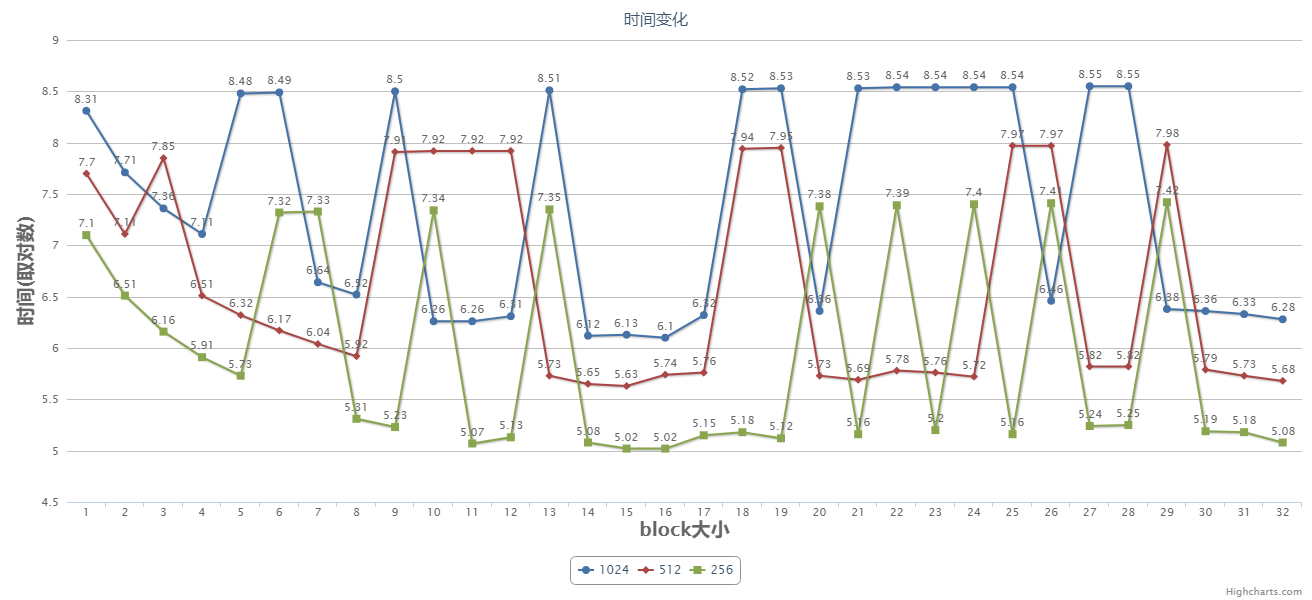
\includegraphics[scale=0.3]{res.png}
    \newline

\section{完整的代码及路径}

\end{CJK}
\end{document}
